\section{Model}
\label{sec:model}
As evidenced by, for example, the Heartbleed and Shellshock vulnerabilities, a single commit, sometimes even a single line of code, can cause a large-scale security problem.  As a consequence, software development teams are investigating the use of security practices in software development. 

We conjecture that a team’s ability to plan, change, and review their codebase, change by change and line by line, is related to their ability to produce secure software.

When presented with lists of the hundreds of software development security practices available (e.g. those listed in the `Building Security in Maturity Model ~\cite{mcgraw2013bsimm} (BSIMM)), the first question industry practitioners typically ask is `Where do I start?'  To answer this question requires a theory for how software development security practices affect the software, as well as an understanding of what the questioner's most significant security problems are. We, further, require enough empirical evidence for the theory to characterize the answers in the context of the person asking the question. In this section, we present a theory of how security practice use affects security outcomes in software development. We express the theory as a model, to support collection of the data needed to test the theory empirically. Ultimately, our goal is to provide evidence-based answers for questions like `Where do I start?', `What do I do next?', and `When do we stop?'.

To underpin the experience and theories bearing on these questions, we propose collecting and analyzing empirical evidence for security practice use and security outcomes in software development. 

From prediction to explanation...

Start with VPM
While we aim to build an explanatory model, we draw from past experience with vulnerability prediction models
Typical VPM: predict vulns (external, CVE) in terms of a set of metrics - SLOC, Churn, ….
We want to add information about what was done to produce the SLOC, etc across the SDLC so we can understand, explain, intervene
We expand the basic prediction model format in two ways


We draw on research in defect prediction and vulnerability prediction to identify and select metrics for measuring security outcomes and criticality.  For example, the relationship between code size and vulnerability is well-established. How does security practice use moderate that relationship?  For example, does the use of coding standards correlate with less vulnerabilities for a given code size? Can thorough testing mitigate a lack of coding standards? Can static analysis substitute for thorough testing? And the situation is more complicated than the examples given; there are factors beyond code size that contribute to vulnerabilities, and security practice use does not prevent all vulnerabilities.  

Modeling section (Just enough modeling to be dangerous)
Statistical literature references three categories of models; descriptive, predictive, and explanatory. 
[Explanatory as distinguished from predictive, descriptive a theory for how practices affect software development]
[Need latent variable motivation, definition]
We construct our model in light of a) explanatory in terms of purpose, evaluated via structural equation modeling in terms of analysis technique.

Sanders~\cite{sanders2009security} argues that existing security metrics should be integrated to provide a comprehensive, quantified view of systems through their lifecycle. Landwehr~\cite{landwehr2015we} argues that secure coding requirements should have a basis in theory or experiment for each requirement. Given the wide variety of security measurements and practices available, a model of the variables and relationships involved in measuring security in software development could help clarify how security practices affect security outcomes. 

what is the effect of a practice?
To model the effect of security practice use on security outcomes in software development, the model must include notions of software, security, practice use, outcomes, and software development. 
 
\subsection{Constructs}
Given our goal of measuring security practice use on software vulnerabilities, we need to model three things; security practice use, software, and vulnerabilities.  We first define conceptual constructs to model each of these things; Adherence, Criticality, and Outcomes then define our approach to measuring each construct.
\subsubsection{Outcomes}
\label{sec:model_contruct_outcome}
The Outcomes construct represents security outcomes for the software. Meneely~\cite{meneely2016security} observes that security is negatively defined, the absence of issues in a system's confidentiality, integrity, and availability. 
However, at present, the presence of security issues, termed vulnerabilities, is the most common means of measuring security in software~\cite{morrison2014mapping}.
To describe the Outcomes construct, we begin with a definition of vulnerability. Following Krsul~\cite{krsul1998software} and Ozment~\cite{ozment2007vulnerability}, we define a software vulnerability as “an instance of a mistake in the specification, development, or configuration of software such that its execution can violate the explicit or implicit security policy. 

The absence of vulnerabilities may only be apparent, due to undiscovered or unreported vulnerabilities in the software. We distinguish between undiscovered (`latent') and discovered (`manifest') security issues.  Vulnerabilities may be manifest, when discovered by users, security researchers or the development team itself, or they may be latent, not yet discovered by users, researchers or the team. We further distinguish between vulnerabilities identified after the software is released (`Post-release'), and vulnerabilities identified before the software is released (`Pre-release'). Pre-release vulnerabilities are an indication that the development team has incorporated practices supporting discovery of vulnerabilities into its development process. Post-release vulnerabilities are an indication of both vulnerabilities that have escaped the development process and of attacker interest in the software. 

We measure the Outcomes construct in terms of manifest vulnerabilities and the  timing of their discovery and resolution. Low total values for manifest vulnerabilities are preferable, and a high proportion of vulnerabilities discovered pre-release rather than post-release is also preferable. 

\subsubsection{Adherence}
The Adherence construct represents the effort the team takes to prevent and discover vulnerabilities. We adapt an IEEE definition of practice~\cite{ieee1990glossary} `3. a specific type of professional or management activity that contributes to 
the execution of a process and that may employ one or more techniques and tools' to define a software development security practice to be an action a software development team member takes to prevent, identify, or resolve a vulnerability, possibly guided by a tool or reference. The Adherence construct is measured in terms of the frequency and prevalence of security practice use by the team. To measure frequency, we count instances of practice use, proportional to total team effort. To measure prevalence, we compute the ratio of team members who apply the practice to total team members. We measure adherence for each security practice to enable comparison of the relative values of the various security practices to which a team adheres.

\subsubsection{Criticality}
The Criticality construct represents the characteristics of the software's purpose, construction, and environment that may affect security Outcomes. To accurately measure Adherence requires accounting for Criticality. For example, a carefully-written piece of widely-used software that manages financial data (high Criticality) may have poorer Outcomes than a less well written baseball scores program used by a few hundred users (low Criticality). The Criticality construct is measured in terms of a set of context factors, associated with each project, that represent factors historically associated with high security risk. 

We hypothesize that the three constructs are related; We expect that both Adherence and Criticality influence Outcomes.  We also expect a relationship between Adherence and Criticality.  In an ideal world, we would expect Adherence to be driven by Criticality, as teams adopted security practices in proportion to the security needs of their software, its environment, and their users. In the real word, users (especially attackers) sometimes surprise development teams in the uses of their software, unexpectedly increasing the software's Criticality out of proportion to the team's Adherence. Figure~\ref{fig:model_constructs} depicts the basic construct relationships. Each circle in the figure represents a construct, modeled as a `latent variable', We model the constructs using latent variables to indicate that our measures for each construct are aggregates of observed variables containing some level of measurement error with respect to the construct ~\cite{kline2015principles,borsboom2008latent}. Each directed edge in the graph represents the influence of one construct upon another, as measured by their covariance. The weights on each edge in figure~\ref{fig:model_constructs} are from simulated data, but they represent the direction of the relationships we expect to see in empirical data, with, for example, increases in adherence leading to reductions in outcomes. 

\begin{figure}
		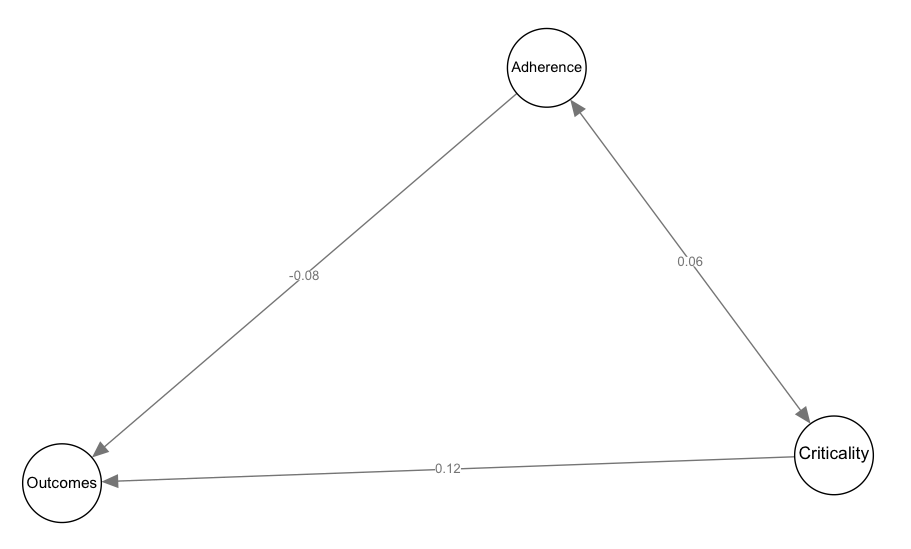
\includegraphics[width=\columnwidth]{modelzero}
	\caption{Model Constructs}
	\label{fig:model_constructs}
\end{figure}

\subsection{Situating the Constructs in Software Development}

To measure Outcomes, Adherence, and Criticality in the context of the software development lifecycle, we need to describe the components of software development in which vulnerabilities are introduced and found, to which security practices are applied, and by which the software may be attacked.   Vulnerabilities may not only be problems in code (`bugs'~\cite{mcgraw2006software}) but may also be, for example, design issues (`flaws'), documentation issues, and configuration issues. We define a set of vulnerability sources, based on the definition of vulnerability we have adopted~\ref{sec:model_contruct_outcome}:  
 \begin{itemize}
 	\item \textbf{Specification} - All activities, e.g. planning, preparation, requirements definition, and design that precede, chronologically or conceptually, coding. 
 	\item \textbf{Coding} - The development and maintenance of software features.
 	\item \textbf{Testing} - The quality assurance activities applied to developed software before it is released.
 	\item \textbf{Operations} - The configuration and use of the released software, and feedback from the software's users to the development organization.
 \end{itemize} 
The vulnerability locations may also be viewed chronologically, as development phases. Boehm ~\cite{boehm1981economics} reports that the earlier in the development process a defect is resolved, the cheaper it is to resolve. We can use data collected according to this scheme to analyze whether vulnerabilities follow the same cost pattern as defects. While many projects will have a more detailed set of development process phases, we conjecture that these phases are present in the majority of software development projects.

As a refinement of the basic constructs model from figure~\ref{fig:model_constructs}, we incorporate the phases into the construct model, as illustrated in \label{fig:model_constructs_phases}

\begin{figure}
	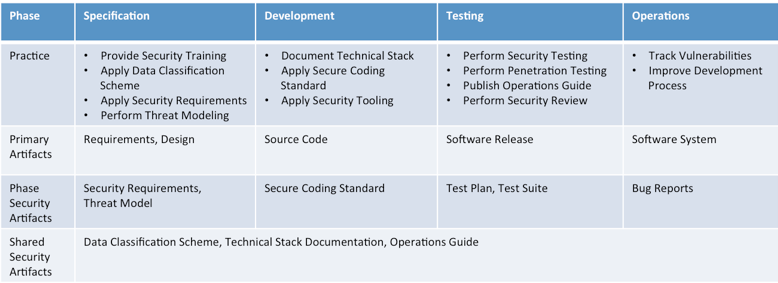
\includegraphics[width=\columnwidth]{PracticesDiagram}
	\caption{Model Constructs and Phases}
	\label{fig:model_constructs_phases}
\end{figure}


\subsection{The Security Practices Evaluation Framework}

To collect empirical data to test the constructs and their relationships, we have developed a data collection framework for the model, available online~\cite{morrison2016spefsite}.   We now present the data elements from the data collection framework. To ground the model and the present study, we include a hypothesis for each data element, which serves as both our reason for its inclusion in the framework and a testable component of the model. We collect Context Factors to measure Criticality, Practice Adherence Metrics to measure Adherence, and Outcome Measures to measure Outcomes.
\subsubsection{Context Factors}
\label{sec:model_cf}

Drawing conclusions from empirical studies in software engineering is difficult because the results of  any process largely depend upon the relevant context variables. One cannot assume a priori that a study’s results generalize beyond the specific environment in which it was conducted [5???]. Therefore, recording a study’s context factors is essential to understanding the generality and utility of the conclusions as well as the similarities and differences between the case study and one’s own environment. Dyba et al. ~\cite{dyba2012what} suggests the question “Does the inclusion of this information explain the constraints on, or the opportunities for, the phenomenon I am studying?” as a guide for including context factors. Jones~\cite{jones2000software} suggests six categories of measurements to be collected for every project; software classification, sociological, project-specific, ergonomic, technological, and international. SP-EF includes the following context factors:
\begin{itemize}
\item \textit{Language} – Language in which the software artifact being measured is written, e.g. Java, C, C++, Python, PHP. \textit{Hypothesis}: Because languages vary in how much access they provide to system memory and hardware, language choice influences security criticality.
\item \textit{Operating System} - Operating system(s) on which the software runs, e.g. Linux, Windows, iOS. \textit{Hypothesis}: Because operating systems vary in how much access they provide to system memory and hardware, and because they reduce an attacker’s effort by presenting a single interface to the population of machines they are available on (monoculture), operating system choice influences security criticality.
\item \textit{Domain} – A description of the software’s purpose, e.g. application, framework, utility. 
\textit{Hypothesis}: Because software domain influences who uses the software, what access to system resources the software has, and how often the software is run software domain influences security criticality.
\item \textit{Product Age} – Number of years since the software began development. 
\textit{Hypothesis}: Because attack and defense techniques for software change over time, product age influences software performance and software criticality.
\item \textit{Source Lines of Code (SLOC)} - Total number of source lines of code (no comments, no blanks) as counted, for example, by the cloc or SLOCCount utilities. 
\textit{Hypothesis}: Because each line of code is an opportunity to make a mistake,  and because code size correlates with other measures of software complexity~\cite{herraiz2009statistical},  SLOC is positively correlated with security criticality.
\item \textit{Churn} – Total number of SLOC added, deleted, or changed during the measurement time period. 
\textit{Hypothesis}: Because changed code is correlated with defects, and even single-line changes   can cause vulnerabilities, Churn is positively correlated with security criticality.
\item \textit{Team size} – Total number of unique individuals in each of the following roles: Manager, Developer, and Tester. \textit{Hypothesis}: Team size is beneficial in enabling appropriate time and effort invested in its requirements, design, implementation, review, testing and documentation activities. Team size is detrimental in terms of knowledge transfer and training requirements. Team size is positively correlated with practice adherence, and influences security outcomes. Through management awareness, security criticality influences Team size.
\item \textit{Team Location} – Team Location indicates whether the team is collocated or distributed. \textit{Hypothesis}: Because knowledge transfer and team cohesion are affected by team distribution, Team Location influences practice adherence.
\item \textit{Methodology} – Software development process approach used by team. \textit{Hypothesis}: Because the degree of effort put in to software process planning, documentation, and controls supports control over the delivered software and consumes team resources, Methodology influences practice adherence and security outcomes.
\item \textit{Number of Machines} - Number of machines is a count of how many machines on which the software is installed. The rise of botnets, networks of computers that can be centrally directed, has created a black market for their services.  In 2013, an hour of machine time on a botnet ranged from 2.5 – 12 US cents , and so the number of machines a piece of software runs on is a risk factor. \textit{Hypothesis}: Because economies of scale and monoculture work to the benefit of attackers as well as providers, Number of Machines is positively correlated with security criticality.
\item \textit{Number of Identities} - Number of identities is a count of how many individuals data are managed by the software.  In 2011, a personal identity could be bought (in groups of 1000) for 16 US cents  , and so the number of identities a piece of software manages is a risk factor. \textit{Hypothesis}: Because economies of scale work to the benefit of attackers as well as providers, Number of Identities is positively correlated with security criticality.
\item \textit{Confidentiality, Integrity, and Availability Requirement} (from CVSS) – The CVSS specification includes three data elements, one for each of Confidentiality, Integrity, and Availability, for indicating the security sensititivty of data. The values for each element are subjective assessments of the most sensitive data that passes through, or is kept by, the software under consideration for its Confidentiality (CR), Integrity (IR), and Availability (AR) requirements. \textit{Hypothesis}: Because CR, IR, and AR describe the security importance of the software, they are positively correlated with security criticality.
\item \textit{Source Code Avalability} – Source Code Availability indicates whether the software is proprietary or open source. \textit{Hypothesis}: Anderson [ref] showed that Source Code Availability influences security criticality and practice adherence in both positive and negative ways, depending on project specifics.
\end{itemize}

\subsubsection{Practice Adherence Metrics}
Researchers have empirically evaluated software development practices for their security benefits, for example, in requirements engineering~\cite{riaz2014hidden}, design patterns~\cite{uzunov2015comprehensive}, threat modeling~\cite{shostack2014threat}, static and dynamic analysis~\cite{austin2013comparison}, code review~\cite{meneely2014empirical}, testing~\cite{austin2013comparison}, and attack surface analysis~\cite{theisen2015approximating}.

Different projects are unlikely to use the same set of security practices, or to use a given security practice in exactly the same way. Project teams may adapt their methodology through adding and dropping practices to suit the requirements of their customers, their business and operational environments, and their awareness of trends in software development. Adherence metrics are a means of characterizing the degree to which a practice is used on a project. 
We have included subjective and objective metrics for measuring practice adherence. People are the driving force behind process and practices, and their views should be considered. We adopt four measures from UTAUT ~\cite{venkatesh2003user}, a model for the study of technology adoption, and add a fifth measure to support measurement of productivity: 
\begin{itemize}
\item \textit{Usage} - How often is this practice applied? \textit{Hypothesis}: Usage is a direct measure of the frequency of the use of a practice, positively correlated with practice adherence.
\item \textit{Ease Of Use} - How easy is this practice to use? \textit{Hypothesis}: Ease of Use is positively correlated with practice adherence.
\item \textit{Utility} - How much does this practice assist in providing security in the software under development? \textit{Hypothesis}: Utility is positively correlated with practice adherence.
\item \textit{Training} - How well trained is the project staff in the practices being used? \textit{Hypothesis}: Training is positively correlated with practice adherence.
\item \textit{Effort} - How much time, on average, does applying this practice take each time you apply it? \textit{Hypothesis}: Effort is a direct measure of practice adherence.
\end{itemize}
To support triangulation with subjective metrics, and support for studies where the team is unavailable, we define the following objective practice adherence metrics:
\begin{itemize}
\item \textit{Frequency}: Number of references to the practice, obtained by researcher observation and/or text mining. \textit{Hypothesis}:  How frequently practices are mentioned in project documentation and history is correlated with practice adherence.
\item \textit{Prevalence}: Proportion of the team applying the practice, the ratio of all practice users to all team members. \textit{Hypothesis}: Many studies, e.g. Venkatesh ~\cite{venkatesh2003user} and Witschey ~\cite{witschey2015quantifying}, show use by other team members to be correlated with why developers use practices. \textit{Hypothesis}: Prevalence is positively correlated with practice adherence.
\end{itemize}
For each security practice adherence event, we recorded the following data elements:
\begin{itemize}
\item \textit{Event Date} – Date on which document was created.
\item \textit{Practice} – Name of security practice associated with document. 
\item \textit{Source} – Data source for document. Possible Values: Version Control, Defect Tracker, Email.
\item \textit{Document Id} – Id of document in its source, e.g. commit hash, bug tracker id, email id.
\item \textit{Creator} – Author of the source document.
\item \textit{Assignee} – For defect report documents, the person assigned the defect, where applicable.
\end{itemize}

While the practice adherence metrics are not tied to a specific set of practices, we have defined a set of software development security practices, synthesized from the BSIMM, SDL, SAFECode, and OWASP practice lists.  

From our definition, we define a template for describing security practice use: <Role>(team member)<Verb>(action)<Artifact(s) Affected>, (guided by)<Artifact(s) Referenced>. We read through the BSIMM, SDL, SAFECode, and OWASP practice lists, filling out the template for each security practice. We identifying 16 practices that, in combination with roles (e.g. Manager, Developer), verbs (e.g. ‘implement’, ‘test’, ‘document’) , phases (e.g. ‘Design’, ‘Testing’), and artifacts (e.g. ‘Requirements’, ‘Source Code’, ‘Regulations’), were sufficient to classify the source practices we identified. We excluded three of the practices, ‘Apply Security Principles’,  ‘Monitor Security Metrics’ and ‘Publish Disclosure Policy’ from the framework because they were mentioned less than 2\% of the time across our sources.
Once we had classified the practices, we revisited the text of the source practices, and extracted representative keywords and questions characterizing how the practice is implemented. 
 Table 1 lists the practices, with descriptions, and keywords for each practice. Documentation for all of the roles, verbs, phases, artifacts, keywords, and questions is available at the website~\cite{morrison2016spefsite}.

\subsubsection{Outcome Measures}
In this section, we describe the set of attributes and values that are used to describe the security-related outcomes of the project. 

While hundreds of security metrics have been proposed~\cite{rudolph2012critical},~\cite{verendel2009quantified}, tracking a relatively small set of attributes for each vulnerability detected in the software is sufficient to replicate many of them. In addition to data kept for defects (e.g. those attributes listed by Lamkanfi et al.  ~\cite{lamkanfi2013eclipse}), we collect:
\begin{itemize}
\item \textit{Source} – The name of the bug tracker or bug-tracking database where the vulnerability is recorded.
\item \textit{Identifier} – The unique identifier of the vulnerability in its source database.
\item \textit{Description} – Text description of the vulnerability.
\item \textit{Discovery Date} – Date the vulnerability was discovered. 
\item \textit{Creation Date} – Date the tracking record was created.
\item \textit{Patch Date} – The date the change resolving the vulnerability was made.
\item \textit{Release Date} – The date the software containing the vulnerability was released.
\item \textit{Severity} – The criticality of the vulnerability. 
\item \textit{Phase}  – Indication of when during the development lifecycle the vulnerability was discovered
\item \textit{Reporter} – Indication of who found the vulnerability. (Optional) Role Name and/or email address of person in the reporter role. 
\end{itemize}

Given a collection of vulnerabilities with the attributes specified above, we can compute the following measures:
\begin{itemize}
\item \textit{Pre-release Vulnerabilities} - Vulnerabilities found in new and changed code before software is released. \textit{Hypothesis}: The goal of security practice adherence is to avoid releasing software with vulnerabilities, so pre-release vulnerabilities are positively correlated with security effort, and negatively correlated with security outcomes.
\item \textit{Post-release Vulnerabilities} - Vulnerabilities found in new and changed code after software is released. \textit{Hypothesis}: Post-release Vulnerabilities represent a failure of the process to catch vulnerabilities pre-release, and are negatively correlated with security outcomes.
\item \textit{Vulnerability Density} - Vulnerability Density (Vdensity) is the cumulative vulnerability count per unit size of code ~\cite{alhazmi2007assessing}. We adopt a size unit of thousand source lines of code (KSLOC). \textit{Hypothesis}: Vulnerability Density is a derived measure negatively correlated with security outcomes ~\cite{alhazmi2007measuring}.
\item \textit{Vulnerability Removal Effectiveness} - Vulnerability Removal Effectiveness (VRE) is the ratio of pre-release vulnerabilities to total vulnerabilities found, pre- and post-release, analogous to defect removal effectiveness ~\cite{kan2002metrics}. Ideally, a development team will find all vulnerabilities before the software is shipped.  VRE is a measure for how effective the team’s security practices are at finding vulnerabilities before release. \textit{Hypothesis}: VRE is positively correlated with practice adherence, and negatively correlated with security outcomes.
\end{itemize}


\subsection{Putting it all together; three refinements of the model}

In this section, we build three graphical models of the hypothesized relationships described above, representing three levels of measurement detail.

	Draw base C-A-O model
	Add S-C-T-O Ozment comments, picture
	Add (and extract, revise) practices, present full 13 - SCTO - CAO model
	



